\section{Item Pools}\label{sec:itempools}

At the start, the pools are filled according a certain amount of entropy. Here are the random things that can happen.

\begin{wrapfigure}{r}{0.2\textwidth}
   \begin{center}
      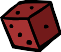
\includegraphics{img/D6.png}
   \end{center}
\end{wrapfigure}


\subsubsection*{Preamble}

The probabilities are represented as a bar filled according to either what item is put in the pool or what pool the item is put in. Here is an example: 
\begin{table}[H]
\resizebox{(\columnwidth)*4/5}{!}{
\begin{tabular}{| p{((\textwidth)*4/5)/3} | p{((\textwidth)*4/5)*2/3} |}
\hline
\cellcolor{orange}Item 1 (33.3\%)& \cellcolor{BrickRed}Item 2 (66.6\%)\\ \hline
\end{tabular}}
\resizebox{(\columnwidth)*4/5}{!}{
\begin{tabular}{| p{((\textwidth)*4/5)*2/3} | p{((\textwidth)*4/5)/3} |}
\hline
\cellcolor{Melon}Item 3 (66.6\%)& \cellcolor{White}Nothing (33.3\%)\\ \hline
\end{tabular}}
\end{table}
Each row corresponds to a diffrent dice throw. Keep in mind that they are, indeed, independant. However, if they are on the same row, they correspond to the same random choice. When a certain area has a white background, then there's a probability that nothing is added.


\subsection{Pool-specific randomization}
In this section, we will look at how the pools are filled with random items.

\subsubsection*{Boss Pool}
\begin{table}[H]
\resizebox{(\columnwidth)*4/5}{!}{
\begin{tabular}{| p{((\textwidth)*4/5)/2} | p{((\textwidth)*4/5)/2} |}
\hline
\cellcolor{orange}The Wooden Spoon (50\%)& \cellcolor{LimeGreen}The Belt (50\%)\\ \hline
\end{tabular}}
\resizebox{(\columnwidth)*4/5}{!}{
\begin{tabular}{| p{((\textwidth)*4/5)/3} | p{((\textwidth)*4/5)/3} | p{((\textwidth)*4/5)/3} |}
\hline
\cellcolor{ProcessBlue}Moms Underwear (33\%)& \cellcolor{SeaGreen}Moms Heels (33\%)& \cellcolor{Thistle}Moms Lipstick (33\%)\\ \hline
\end{tabular}}
\resizebox{(\columnwidth)*4/5}{!}{
\begin{tabular}{| p{((\textwidth)*4/5)/3} | p{((\textwidth)*4/5)/3} | p{((\textwidth)*4/5)/3} |}
\hline
\cellcolor{ProcessBlue}Moms Underwear (33\%)& \cellcolor{SeaGreen}Moms Heels (33\%)& \cellcolor{Thistle}Moms Lipstick (33\%)\\ \hline
\end{tabular}}
\resizebox{(\columnwidth)*4/5}{!}{
\begin{tabular}{| p{(0.625\textwidth)*4/5} | p{(0.3\textwidth)*4/5} |}
\hline
\cellcolor{Lavender}The Bandage (66.6\%)& \cellcolor{White}\\ \hline
\end{tabular}}
\end{table}

Note: There is a $\frac{1}{3}$ chance that Moms Underwear, Moms Heels or Moms Lipstick appears twice in the Boss Room pool.

\subsubsection*{Golden Chests Pool}
\begin{table}[H]
\resizebox{(\columnwidth)*4/5}{!}{
\begin{tabular}{| p{((\textwidth)*4/5)/2} | p{((\textwidth)*4/5)/2} |}
\hline
\cellcolor{orange}The Wooden Spoon (50\%)& \cellcolor{LimeGreen}The Belt (50\%)\\ \hline
\end{tabular}}
\resizebox{(\columnwidth)*4/5}{!}{
\begin{tabular}{| p{((\textwidth)*4/5)/3} | p{((\textwidth)*4/5)/3} | p{((\textwidth)*4/5)/3} |}
\hline
\cellcolor{ProcessBlue}Moms Underwear (33\%)& \cellcolor{SeaGreen}Moms Heels (33\%)& \cellcolor{Thistle}Moms Lipstick (33\%)\\ \hline
\end{tabular}}
\end{table}

\subsubsection*{Secret Room Pool}
\begin{table}[H]
\resizebox{(\columnwidth)*4/5}{!}{
\begin{tabular}{| p{((\textwidth)*4/5)/2} | p{((\textwidth)*4/5)/2} |}
\hline
\cellcolor{VioletRed}2 $\times$ My Little Unicorn and 1up! (50\%)& \cellcolor{SpringGreen}1 $\times$ My Little Unicorn and 1up! (50\%)\\ \hline
\end{tabular}}
\resizebox{(\columnwidth)*4/5}{!}{
\begin{tabular}{| p{(0.625\textwidth)*4/5} | p{((\textwidth)*4/5)/3} |}
\hline
\cellcolor{Emerald}Transcendance (66.6\%)& \cellcolor{White}\\ \hline
\end{tabular}}
\end{table}

\subsubsection*{Shop Pool}
\begin{table}[H]
\resizebox{(\columnwidth)*4/5}{!}{
\begin{tabular}{| p{((\textwidth)*4/5)/2} | p{((\textwidth)*4/5)/2} |}
\hline
\cellcolor{GreenYellow}9V (50\%)& \cellcolor{White}\\ \hline
\end{tabular}}
\resizebox{(\columnwidth)*4/5}{!}{
\begin{tabular}{| p{((\textwidth)*4/5)/2} | p{((\textwidth)*4/5)/2} |}
\hline
\cellcolor{Goldenrod}The Battery (50\%)& \cellcolor{White}\\ \hline
\end{tabular}}
\end{table}

\subsubsection*{Devil Room Pool}
\begin{table}[H]
\resizebox{(\columnwidth)*4/5}{!}{
\begin{tabular}{| p{((\textwidth)*4/5)/3} | p{((\textwidth)*4/5)*2/3} |}
\hline
\cellcolor{Orchid}Lord of The Pit (33.3\%)& \cellcolor{White}\\ \hline
\end{tabular}}
\resizebox{(\columnwidth)*4/5}{!}{
\begin{tabular}{| p{(0.625\textwidth)*4/5} | p{((\textwidth)*4/5)/3} |}
\hline
\cellcolor{Gray}The Nail (66.6\%)& \cellcolor{White}\\ \hline
\end{tabular}}
\end{table}

\subsection{Item-specific randomization}
In this section, we will look at how the items are sorted into random pools.

\begin{table}[H]
\resizebox{(\columnwidth)*4/5}{!}{
\begin{tabular}{| p{((\textwidth)*4/5)/8} | p{((\textwidth)*4/5)/4} | p{((\textwidth)*4/5)/4} | p{((\textwidth)*4/5)/4} |}
\hline
\cellcolor{White}Legend: & \cellcolor{LimeGreen}Regular Room Pool&\cellcolor{Maroon}Devil Room Pool& \cellcolor{Yellow}Secret Room Pool\\ \hline
\end{tabular}}
\end{table}
\begin{table}[H]
\resizebox{(\columnwidth)*4/5}{!}{
\begin{tabular}{| p{(0.4\textwidth)} | p{(0.2\textwidth)} | p{(0.3\textwidth)} |}
\hline
\cellcolor{LimeGreen}\footnotesize{The Necronomicon (44.4\%)}&\cellcolor{Maroon}\scriptsize{The Necronomicon (22.2\%)}& \cellcolor{White}\\ \hline
\end{tabular}}
\resizebox{(\columnwidth)*4/5}{!}{
\begin{tabular}{| p{(0.3\textwidth)} | p{(0.3\textwidth)} | p{(0.3\textwidth)} |}
\hline
\cellcolor{LimeGreen}\footnotesize{We Need to Go Deeper (33.3\%)}&\cellcolor{Maroon}\footnotesize{We Need to Go Deeper (33.3\%)}& \cellcolor{White}\\ \hline
\end{tabular}}
\resizebox{(\columnwidth)*4/5}{!}{
\begin{tabular}{| p{(0.73\textwidth)} | p{(0.18\textwidth)} |}
\hline
\cellcolor{LimeGreen}\footnotesize{Technology (80\%)}&\cellcolor{Maroon}\footnotesize{Technology (20\%)}\\ \hline
\end{tabular}}
\resizebox{0.8\columnwidth}{!}{
\begin{tabular}{| p{(0.3\textwidth)} | p{(0.3\textwidth)} | p{(0.3\textwidth)} |}
\hline
\cellcolor{LimeGreen}\footnotesize{The Book of Belial (33.3\%)}&\cellcolor{Maroon}\footnotesize{The Book of Belial (33.3\%)}& \cellcolor{Yellow}\footnotesize{The Book of Belial (33.3\%)}\\ \hline
\end{tabular}}
\resizebox{0.8\columnwidth}{!}{
\begin{tabular}{| p{(0.3\textwidth)} | p{(0.625\textwidth)} |}
\hline
\cellcolor{LimeGreen}\footnotesize{The Lucky Foot (33.3\%)}&\cellcolor{Maroon}\footnotesize{Lucky Foot (66.6\%)}\\ \hline
\end{tabular}}
\resizebox{(\columnwidth)*4/5}{!}{
\begin{tabular}{| p{(0.625\textwidth)} | p{(0.3\textwidth)} |}
\hline
\cellcolor{LimeGreen}\footnotesize{A Quarter (66.6\%)}&\cellcolor{Maroon}\footnotesize{A Quarter (33.3\%)}\\ \hline
\end{tabular}}
\resizebox{(\columnwidth)*4/5}{!}{
\begin{tabular}{| p{(0.625\textwidth)} | p{(0.3\textwidth)} |}
\hline
\cellcolor{LimeGreen}\footnotesize{The Book of Sin (66.6\%)}&\cellcolor{Maroon}\footnotesize{The Book of Sin (33.3\%)}\\ \hline
\end{tabular}}
\resizebox{(\columnwidth)*4/5}{!}{
\begin{tabular}{| p{(0.625\textwidth)} | p{(0.3\textwidth)} |}
\hline
\cellcolor{LimeGreen}\footnotesize{The Common Cold (66.6\%)}&\cellcolor{Maroon}\footnotesize{The Common Cold (33.3\%)}\\ \hline
\end{tabular}}
\resizebox{(\columnwidth)*4/5}{!}{
\begin{tabular}{| p{(0.625\textwidth)} | p{(0.3\textwidth)} |}
\hline
\cellcolor{LimeGreen}\footnotesize{The Parasite (66.6\%)}&\cellcolor{Maroon}\footnotesize{The Parasite (33.3\%)}\\ \hline
\end{tabular}}
\resizebox{(\columnwidth)*4/5}{!}{
\begin{tabular}{| p{(0.625\textwidth)} | p{(0.3\textwidth)} |}
\hline
\cellcolor{LimeGreen}\footnotesize{Money=Power (66.6\%)}&\cellcolor{Maroon}\footnotesize{Money=Power (33.3\%)}\\ \hline
\end{tabular}}
\resizebox{(\columnwidth)*4/5}{!}{
\begin{tabular}{| p{(0.625\textwidth)} | p{(0.3\textwidth)} |}
\hline
\cellcolor{LimeGreen}\footnotesize{Demon Baby (66.6\%)}&\cellcolor{Maroon}\footnotesize{Demon Baby (33.3\%)}\\ \hline
\end{tabular}}
\resizebox{(\columnwidth)*4/5}{!}{
\begin{tabular}{| p{(0.625\textwidth)} | p{(0.3\textwidth)} |}
\hline
\cellcolor{LimeGreen}\footnotesize{Forget Me Now (66.6\%)}&\cellcolor{Maroon}\footnotesize{Forget Me Now (33.3\%)}\\ \hline
\end{tabular}}
\resizebox{(\columnwidth)*4/5}{!}{
\begin{tabular}{| p{(0.625\textwidth)} | p{(0.3\textwidth)} |}
\hline
\cellcolor{LimeGreen}\footnotesize{Monster Manual (66.6\%)}&\cellcolor{Maroon}\footnotesize{Monster Manual (33.3\%)}\\ \hline
\end{tabular}}
\end{table}

\subsubsection*{Notes}
\noindent \textbf{Necronomicon}: If the Necronomicon falls in the white space, it won't even appear in the Library Pool.

\noindent \textbf{The Book of Sin, The Book of Belial and The Monster Manual} always are in the Library Pool.

\noindent \textbf{The Book of Belial}: If playing with Judas, it won't be put in any pool (including the Library Pool).

\noindent \textbf{Lucky Foot}: It seems that Cain can find it. I haven't found the mechanism that prevents him to do so.

\subsubsection*{Other specific rules}

\begin{table}[H]
\resizebox{(\columnwidth)*4/5}{!}{
\begin{tabular}{| m{((\textwidth)*4/5)/2} | m{((\textwidth)*4/5)/2} |}
\hline
\cellcolor{RedOrange}(1) Holy Grail/Bum Friend (50\%)&\cellcolor{Periwinkle}(2) Portable Slot Machine (50\%)\\ \hline
\end{tabular}}
\resizebox{(\columnwidth)*4/5}{!}{
\begin{tabular}{| m{((\textwidth)*4/5)/2} | m{((\textwidth)*4/5)/2} |}
\hline
\cellcolor{JungleGreen}(3) Fate/Pyro! (50\%)&\cellcolor{White}\\ \hline
\end{tabular}}
\end{table}

\begin{enumerate}[(1) :]
\item The God Room Pool contains Holy Grail \textit{and} the Shop Pool contains Bum Friend (if not (2)).
\item The Shop Pool contains The Portable Slot Machine (if not (1)).
\item The Golden Chest Pool contains Fate \textit{and} the Secret Room Pool contains Pyro!
\end{enumerate}

\subsection{Post-processing}
After that, all the items in the Boss Pool, Shop Pool and Golden Chest Pool are removed from the Regular Pool.

\subsection{Code where it happens}
See lines 9885 to ??? from the source code.
